\documentclass[11pt]{article}
\usepackage{geometry,marginnote} % Pour passer au format A4
\geometry{hmargin=1cm, vmargin=1cm} % 

% Page et encodage
\usepackage[T1]{fontenc} % Use 8-bit encoding that has 256 glyphs
\usepackage[english,french]{babel} % Français et anglais
\usepackage[utf8]{inputenc} 

\usepackage{lmodern,numprint}
\setlength\parindent{0pt}

% Graphiques
\usepackage{graphicx,float,grffile,units}
\usepackage{tikz,pst-eucl,pst-plot,pstricks,pst-node,pstricks-add,pst-fun,pgfplots} 

% Maths et divers
\usepackage{amsmath,amsfonts,amssymb,amsthm,verbatim}
\usepackage{multicol,enumitem,url,eurosym,gensymb,tabularx}

\DeclareUnicodeCharacter{20AC}{\euro}



% Sections
\usepackage{sectsty} % Allows customizing section commands
\allsectionsfont{\centering \normalfont\scshape}

% Tête et pied de page
\usepackage{fancyhdr} \pagestyle{fancyplain} \fancyhead{} \fancyfoot{}

\renewcommand{\headrulewidth}{0pt} % Remove header underlines
\renewcommand{\footrulewidth}{0pt} % Remove footer underlines

\newcommand{\horrule}[1]{\rule{\linewidth}{#1}} % Create horizontal rule command with 1 argument of height

\newcommand{\Pointilles}[1][3]{%
  \multido{}{#1}{\makebox[\linewidth]{\dotfill}\\[\parskip]
}}

\newtheorem{Definition}{Définition}

\usepackage{siunitx}
\sisetup{
    detect-all,
    output-decimal-marker={,},
    group-minimum-digits = 3,
    group-separator={~},
    number-unit-separator={~},
    inter-unit-product={~}
}

\setlength{\columnseprule}{1pt}

\begin{document}

\textbf{Nom, Prénom :} \hspace{8cm} \textbf{Classe :} \hspace{3cm} \textbf{Date :}\\
\vspace{-0.8cm}
\begin{center}
  \textit{La normalité est une route pavée : on y marche aisément mais les fleurs n’y poussent pas.} - \textbf{Vincent Van Gogh}
\end{center}
\vspace{-0.8cm}

\subsection*{Définition}

$x$ est \dotfill \\ \Pointilles[1]

\subsection*{Equations}


\begin{multicols}{2}
\begin{itemize}[label={$\bullet$}]
\item $4x + 10 = 128$ \\ \Pointilles[10]  \columnbreak 
\item $6x - 12 = 258$ \\ \Pointilles[10]
\end{itemize} 
\end{multicols}

\begin{multicols}{2}
  \begin{itemize}[label={$\bullet$}]
\item $-2x - 12 = -42$ \\ \Pointilles[10]  \columnbreak 
\item $-3.2x + 120 = 43$ \\ \Pointilles[10]
\end{itemize} 
\end{multicols}

\begin{multicols}{2}
  \begin{itemize}[label={$\bullet$}]
\item $15 + 12x = 120 $ \\ \Pointilles[10]  \columnbreak 
\item $3500 = 2400 + 6x$ \\ \Pointilles[10]
\end{itemize} 
\end{multicols}

\begin{multicols}{2}
  \begin{itemize}[label={$\bullet$}]
\item $280 = -70 - 10x$ \\ \Pointilles[10]  \columnbreak 
\item $0.4 - 6.5x = 3.22$ \\ \Pointilles[10]
\end{itemize} 
\end{multicols}

\begin{multicols}{2}
  \begin{itemize}[label={$\bullet$}]
\item $4x + \dfrac{20}{3} = \sqrt{20}$ \\ \Pointilles[10]  \columnbreak 
\item $x \times 2.4 \times 10^{9} +  2.4 \times 10^{12} = 3.6 \times 10^{13}$ \\ \Pointilles[10]
\end{itemize} 
\end{multicols}

\begin{figure}[H]
  \centering
  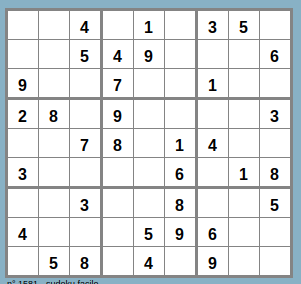
\includegraphics[width=0.6\linewidth]{4x6-equations/sudoku-9a.png}
\end{figure}

\newpage


\textbf{Nom, Prénom :} \hspace{8cm} \textbf{Classe :} \hspace{3cm} \textbf{Date :}\\
\vspace{-0.8cm}
\begin{center}
  \textit{La normalité est une route pavée : on y marche aisément mais les fleurs n’y poussent pas.} - \textbf{Vincent Van Gogh}
\end{center}
\vspace{-0.8cm}

\subsection*{Définition}

$x$ est \dotfill \\ \Pointilles[1]

\subsection*{Equations}


\begin{multicols}{2}
\begin{itemize}[label={$\bullet$}]
\item $6x - 10 = 128$ \\ \Pointilles[10]  \columnbreak 
\item $8x + 12 = 258$ \\ \Pointilles[10]
\end{itemize} 
\end{multicols}

\begin{multicols}{2}
  \begin{itemize}[label={$\bullet$}]
\item $-4x + 14 = -42$ \\ \Pointilles[10]  \columnbreak 
\item $-6.2x - 120 = -143$ \\ \Pointilles[10]
\end{itemize} 
\end{multicols}

\begin{multicols}{2}
  \begin{itemize}[label={$\bullet$}]
\item $25 + 16x = 320 $ \\ \Pointilles[10]  \columnbreak 
\item $6400 = 1800 + 8x$ \\ \Pointilles[10]
\end{itemize} 
\end{multicols}

\begin{multicols}{2}
  \begin{itemize}[label={$\bullet$}]
\item $480 = -50 - 10x$ \\ \Pointilles[10]  \columnbreak 
\item $0.8 - 3.2x = 6.33$ \\ \Pointilles[10]
\end{itemize} 
\end{multicols}

\begin{multicols}{2}
  \begin{itemize}[label={$\bullet$}]
\item $5x + \dfrac{21}{7} = \sqrt{40}$ \\ \Pointilles[10]  \columnbreak 
\item $x \times 2.6 \times 10^{8} +  2.8 \times 10^{13} = 4.6 \times 10^{12}$ \\ \Pointilles[10]
\end{itemize} 
\end{multicols}

\begin{figure}[H]
  \centering
  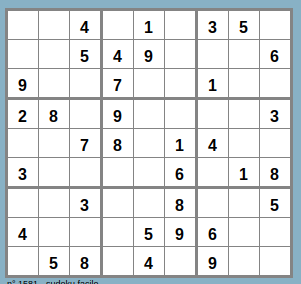
\includegraphics[width=0.6\linewidth]{4x6-equations/sudoku-9a.png}
\end{figure}

\end{document}